\section{Alert Production}
\label{sec:ap}



Alert Production is run each night to produce catalogs and images for sources that have varied or moved relative to a previous observation.  The data products produced by Alert production are given in  \hyperref[table:ap_data_products]{Table~\ref{table:ap_data_products}}.


\begin{table}[htb]
\small
\begin{tabularx}{\textwidth}{ | l | l | X | }
  \hline
  \textbf{Name} & \textbf{Availability} & \textbf{Description} \\
  \hline
  \DIASource & Stored &
  Measurements from difference image analysis of individual exposures. \\
  \hline
  \DIAObject& Stored &
  Aggregate quantities computed by associating spatially colocated \DIASources. \\
  \hline
  DIAForcedSource & Stored &
  Flux measurements on each difference image at the position of a \DIAObject. \\
  \hline
  \SSObject & Stored &
  Solar system objects derived by associating \DIASources and inferring their orbits. \\
  \hline
  CalExp & Stored &
  Calibrated exposure images for each CCD/visit (sum of two snaps) and associated metadata (e.g.\ WCS and estimated background). \\
  \hline
TemplateCoadd & Temporary &
  DCR corrected template coadd. \\
  \hline
  DiffExp & Stored &
  Difference between CalExp and PSF-matched template coadd. \\
  \hline
  VOEvent & Stored &
  Database of VOEvents as streamed from the Alert Production\\
  \hline
 Tracklets & Persisted &
  Intermediate data product for the generation of \SSObjects generated by linking moving sources within a given night \\
  \hline



  \hline
\end{tabularx}
\caption{Table of derived and persisted data products produced during  Alert Production.  A detailed  description of these data products can be found in the Data Products Definition Document \citedsp{LSE-163}.
\label{table:ap_data_products}}
\end{table}

Alert Production is designed as five separate components: single frame processing, alert generation, alert distribution, precovery photometry, and a moving objects pipeline. The first four of these components run as a linear pass through of the data. The moving objects pipeline is run independently of the rest of the alert production. The flow of information through this system is shown in \hyperref[fig:nightly]{Figure~\ref{fig:nightly}}.

\begin{figure}
\begin{center}
\includegraphics[width=0.9\textwidth]{figures/LDM-151_Nightly_Overview.png}
\caption{\label{fig:nightly} The alert production flow of data through the processing pipelines (single frame processing, alert generation,  alert distribution, precovery photometry) }
\end{center}
\end{figure}

In this document we do not address estimation of the selection function for alert generation through the injection of simulated sources. Such a process could be undertaken in batch mode as part of the DRP. Source detection thresholds can be estimated through the use of sky sources (PSF photometry measurements positioned in areas of blank sky).

\subsection{Single Frame Processing Pipeline (\wbsSFM)}
\label{sec:apSingleFrameProcessing}

The Single Frame Processing (SFM) Pipeline (see Figure~\ref{fig:apSFM}) is responsible for reducing raw or camera-corrected image data to \emph{calibrated exposures}, the detection and measurement of \Sources (using the components functionally  part of the Object Characterization Pipeline), the characterization of the point-spread-function (PSF), and the generation of an astrometric solution for an image. Calibrated exposures produced by the SFM pipeline must possess all information necessary for measurement of source properties by single-epoch Object Characterization algorithms.

Astrometric and photometric calibration requires the detection and measurement of the properties of \Sources on a CCD. Accurate centroids and fluxes for these \Sources require an estimation of the PSF and background, which in turn requires knowledge of the positions of the \Sources on an image. The SFM pipeline will, therefore, iterate over background estimation (see \ref{sec:apPSFBackground}) and source measurement (see \ref{sec:apSourcemeasurement})

The SFM pipeline will be implemented as a flexible framework where new processing steps can be added without modifying the stack code (this would include the ability to process non-crosstalk corrected images should a network outage between the base and processing center result in  only the raw data being available). The pipeline, or a subset of the pipeline, should be capable of being run at the telescope facility during commissioning and operations.

\begin{figure}[th]
\begin{center}
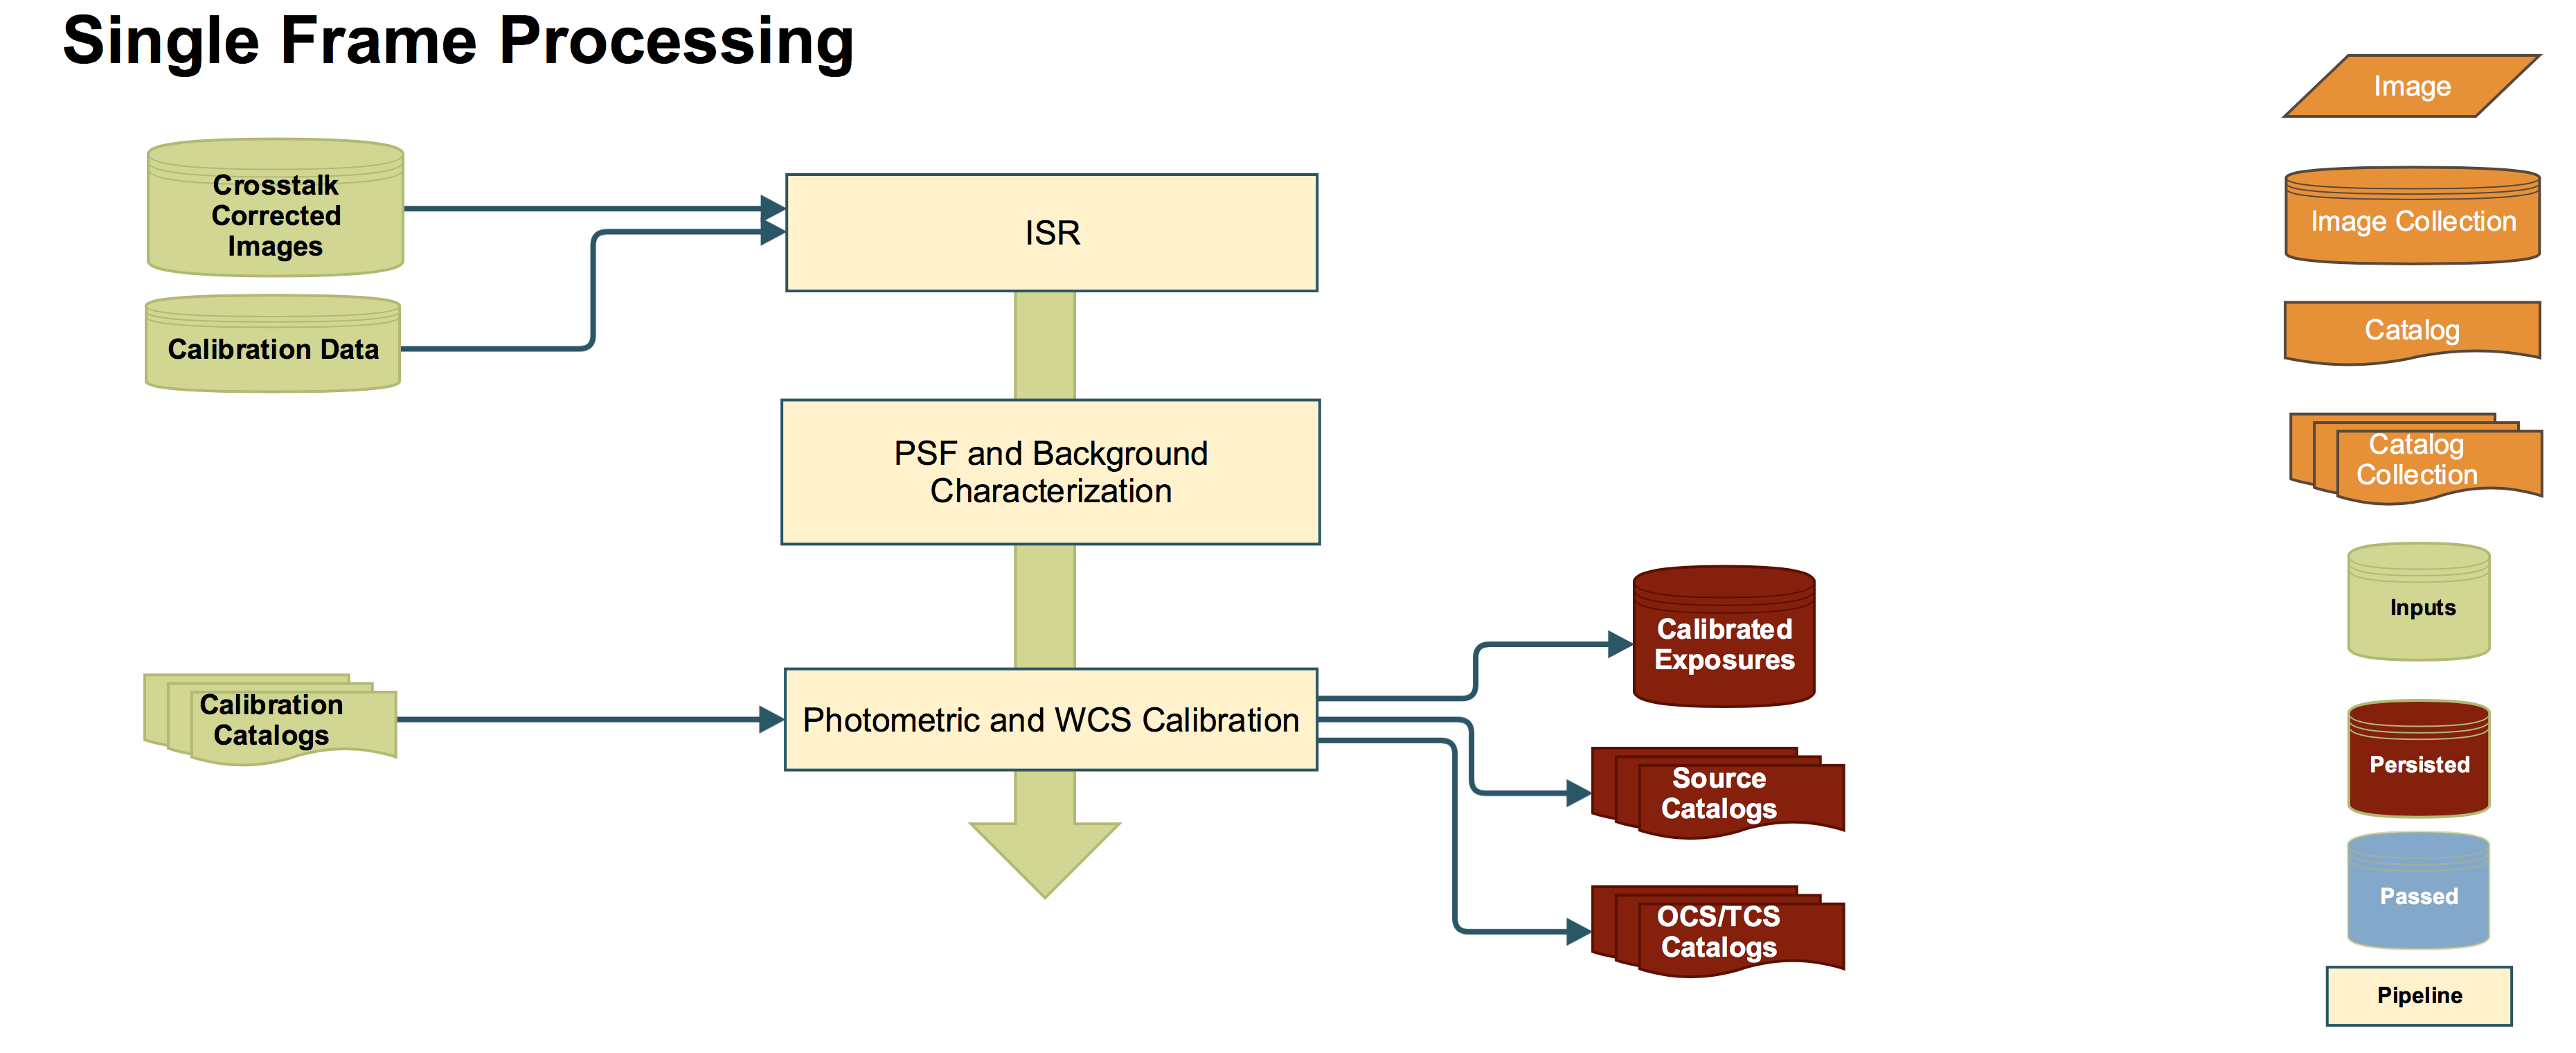
\includegraphics[width=0.9\textwidth]{figures/SFM.png}
\caption{\label{fig:apSFM} Single frame processing of the nightly data: instrument signature removal, astrometric and photometric calibration, background and PSF estimation from the cross-talk corrected camera images.}
\end{center}
\end{figure}

%SFM pipeline functions include:
%\begin{itemize}
%\item Assembly of per-amplifier images to an image of the entire CCD;
%\item Instrumental Signature Removal;
%\item Cosmic ray rejection and snap combining;
%\item Per-CCD determination of zeropoint and aperture corrections;
%\item Per-CCD PSF determination;
%\item Per-CCD WCS determination and astrometric registration of images;
%\item Per-CCD sky background determination;
%\item Source detection and measurement on single frame images
%\item Generation of metadata required by the OCS
%\end{itemize}

\subsubsection{Input Data}
\label{sec:apSFMinput}

\paragraph*{Raw Camera Images:} Amplifier images that have been corrected for crosstalk and bias by the camera software. All images from a visit should be available to the task (including snaps). An approximate WCS is assumed to be available as metadata derived from the Telescope Control System with an absolute pointing uncertainty (for a full focal plane) of 2 arcseconds (OSS-REQ-0298) and the field rotation known to an accuracy of 32 arcseconds (LTS-206).
%\begin{note} question into Steve R about Camera operations - DM to provide request for operations on images that camera team will undertake \end{note}

\paragraph*{Reference Database:} A full-sky astrometric and photometric reference catalog of stars derived either from an external dataset (e.g.\ Gaia) or from the Data Release Processing. Given the current Gaia data release timeline the initial reference catalog is expected to have an astrometric uncertainty of $<0.5$ milliarcseconds and a photometric uncertainty of $<$20 millimag (for a $V=19$ G2V star). The expected release of these calibration catalogs is 2018 and will be derived from the Gaia spectrophotometric observations of non-variable sources.

\paragraph*{Calibration Images:} Flat-field calibration images for all passbands and all CCDs appropriate for the time at which the observations were undertaken. No corrections will be made in the flat-fields for non-uniform pixel sizes - the flat-fields will correct to a common  surface brightness. A flat SED will be assumed for all flat field corrections. Fringe frame calibration images scaled to an amplitude derived from the sky background (i.e.\ no sky spectrum will be available).

\paragraph*{Image Metadata:} List of the positions and extents of CCD defects for all CCDs within the focal plane; electronic parameters for all CCDs (saturation limits, readnoise parameters), electronic and physical footprint for the CCDs, linearity functions, models for the variation in the PSF width with source brightness (brighter-fatter), and parameterized models for a component-based  WCS (e.g.\ a series of optical distortion models) as needed.

\subsubsection{Output Data}
\label{sec:apSFMoutput}

\paragraph*{CalExp Images:} A calibrated exposure (CalExp) is an \hyperref[sec:spImagesExposure]{Exposure} object. The CalExp contains the image pixel values, a variance image, a bitwise mask, a representation of the PSF, the WCS (possibly decomposed into separable components), a photometric calibration object, and a model for the  background. For the alert production, it is not anticipated that a model of the per-pixel covariance will be persisted but this will be revisited dependent on the performance of image subtraction and anomaly characterization as described in \ref{sec:apAlertGeneration}.

\paragraph*{Source Databases:} A catalog of \Sources with measured features described in \ref{sec:apSourcemeasurement}.

\paragraph*{OCS Database} A parameterization of the PSF, WCS, photometric zeropoint, and depth for each CCD in a visit. The PSF may be a simplified version (e.g.\ a single Gaussian) of that derived for the Alert production. These data will be made available to the Telescope Control System (TCS) to assess the success of each observation. A limited version of nightly SFM could be run on the summit to generate this information or the  data will be persisted within a database at the data center that will be accessible to the TCS.


\subsubsection{Instrumental Signature Removal}
\label{sec:apISR}
Instrumental Signature Removal characterizes, corrects, interpolates and flags the camera (or raw) amplifier images to generate a flat-fielded and corrected full CCD exposure.

\paragraph{Pipeline Tasks}
\begin{itemize}
\item Mask the image defects at the amplifier level based on the CCD defect lists, and the per CCD saturation limits
\item Assemble the amplifiers into a single frame (masking missing amplifiers)
\item Apply full frame corrections: dark current correction, flat field to preserve surface brightness, fringe corrections. Flat fields will assume a flat spectral energy distribution (SED) for the source. Fringe frames will be normalized by fitting to the observed sky background.
\item Apply pixel level corrections: apply a correction model for brighter-fatter to homogenize the PSF, correct for static pixel size effects based on a model
\item Interpolate across defects and saturated pixels assuming a model for the PSF (with a nominal FWHM). An estimate of the PSF will be needed for this operation (from the TCS/OCS) or interpolation may be needed to be performed at the end of \ref{sec:apPSFBackground}.
\item Apply a cosmic ray detection algorithm as described in \ref{sec:acCosmicRayDetection}
\item Generate a summed and difference image from the individual snaps propagating the union of the mask pixels in each snap
\end{itemize}

Dependent on the properties of the delivered LSST image quality for 15 second snaps it may be required to model any bulk motion between snaps prior to combination (e.g.\ if dome seeing or the ground layer dominate the lower order components of the seeing).

\subsubsection{PSF and background determination}
\label{sec:apPSFBackground}

Given exposures that have been processed through Instrument Signature Removal, \Sources must be detected to determine the astrometric and photometric calibration of the images. As noted previously an iterative procedure will be adopted to generate an estimate of the background and PSF, and to characterize the properties of the detected sources.  Convergence criteria for this procedure are not currently defined. The default implementation assumes three iterations.

\paragraph{Pipeline Tasks}

The iterative process for PSF and background estimation comprises,
\begin{itemize}
\item Background estimation on the scale of a single CCD is as described in \ref{sec:acBackgroundEstimation}, which divides the CCD into subregions and estimates the background using a robust mean from non-source pixels.
\item Subtraction of the background and the detection of sources as described in \ref{sec:acSourceDetection}. The initial detection threshold for source detection will be 5$\sigma$, with $\sigma$ estimated from variance image plane.
\item Measurement of the properties of the detected sources (see \ref{sec:apSourcemeasurement}). Dependent on the density of sources it may be necessary to deblend the images as described in \ref{sec:acDeblending}
\item Selection of isolated PSF candidate stars based on a signal-to-noise threshold (default 50 $\sigma$). This threshold is significantly deeper than the magnitude limit for Gaia astrometric catalogs but is the threshold at which the astrometric error on the centroid due to photon noise is less than 10 mas and the photometric noise is less than 2\% for the case of the use of a deeper DRP derived reference catalog.
\item Single CCD PSF determination using the techniques described in \ref{sec:acSingleCCDPSF} and the selected bright sources
\item Masking of source pixels within the CCD (growing the footprint of the \Sources to mask the outer regions of the \Source profiles will likely be required to exclude contributes to the background from low surface brightness features).
%\item Single CCD \hyperref[sec:acModelSpatialPSF]{PSF spatial model}
\end{itemize}

The default expectation is that all tasks within this procedure would iterate until convergence.  There maybe significant speed optimizations to be gained by excluding the \Source detection step after an initial detection if the number of sources does not change significantly with updates to the background model.
%\begin{note} Treatment of covariance \end{note}

\subsubsection{Source measurement}
\label{sec:apSourcemeasurement}

For the \Source catalog generated in \ref{sec:apPSFBackground}, source properties are measured using a subset of features described in \ref{sec:acMeasurement}. Source measurement is for all sources within the \Source catalog and not just the bright subset used to calibrate the PSF.  We anticipate using the following plugin algorithms within the \Source measurement step,
\begin{itemize}
\item Centroids based on a static PSF model fit (see \ref{sec:acCentroidAlgorithms} and \ref{sec:acStaticPointSourceModels})
\item Aggregation of pixel flags as described in \ref{sec:acPixelFlags}
\item Aperture Photometry as geven in \ref{sec:acAperturePhotometry} (but only for one or two radii)
\item PSF photometry given in \ref{sec:acStaticPointSourceModels} assuming a static PSF model fit
\item  An aperture correction estimated assuming a static PSF model and measurement of the curve of growth for  detected sources as given in \ref{sec:acApCorr}
\end{itemize}
%\begin{note} why only one or two radii \end{note}

\subsubsection{Photometric and Astrometric calibration}

Photometric and astrometric calibration entails a ``semi-blind'' cross match (because the pointing of the telescope is known to an accuracy of 2 arcseconds) of a reference catalog derived either from the DRP \Objects or from an external catalog (see \ref{sec:apSFMinput}), the generation of a WCS (on the scale of a CCD or full focal plane), and the generation of a photometric zeropoint (on the scale of a CCD). These algorithms must degrade gracefully for the case of larger pointing errors (e.g.\ during the initial calibration of the system during commissioning) and may need to operate in a ``blind'' mode where the pointing and orientation of the telescope is not known.

\paragraph{Pipeline Tasks}

The photometric and astrometric calibration is expected to be performed at the scale of a single CCD. It is possible that the calibration process will need to be extended to larger scales (up to a full focal plane) if there is significant structure in the photometric zero point, or if astrometric distortions cannot be calibrated at the scale of the CCD with sufficient accuracy (i.e.\ the astrometric distortions do not dominate the false positives in the image subtraction). A full focal plane level calibration strategy will introduce synchronization points within the processing of the CCDs as the detections on all CCDs will need to be aggregated prior to the astrometric fit.

The procedures used to match and calibrate the data are,
\begin{itemize}
\item CCD level source association between the DRP reference catalog (or external catalog) and \Sources detected during the PSF and background estimation stage will use a simplified Optimistic B approach described in \ref{sec:acSingleCCDReferenceMatching}. Given an astrometric accuracy of $<0.5$ milliarcseconds from external catalogs such as Gaia (for a $V=19$ G2V star) or  an accuracy of $<50$ milliarcseconds for the DRP catalogs the search radii for sources will be dominated by the uncertainties in the pointing of the telescope and the rotation angle of the camera.
\item Generation of a photometric solution on the scale of a single CCD as described in \ref{sec:acSingleCCDPhotometricFit}
\item Fitting of a WCS astrometric model for a single CCD  using the algorithms given in \ref{sec:acSingleCCDAstrometricFit}. The WCS model is expected to be composed of a sum of transforms or astrometric components (e.g.\ a optical model for the telescope, a lookup table or model for sensor effects such as tree rings).
\item Persistance of the astrometric, PSF, and photometric solutions for possible use by the Telescope Control system (TCS) (see \ref{sec:apSFMoutput})
\end{itemize}

Given the number of stars available on a CCD or the complexity of the astrometric solutions for the LSST (e.g.\ the decomposition of the WCS into components) it may be necessary that the astrometric and photometric solutions be performed for a full focal plane and not just a CCD.  For these cases the algorithms used will be single visit matching (see \ref{sec:acSingleVisitReferenceMatching}),  single visit photometric solutions (see \ref{sec:acSingleCCDPhotometricFit}), and single visit astrometric fits (see \ref{sec:acSingleVisitAstrometricFit}). Fitting to a full focal plane introduces a synchronization point in the alert processing where all CCDs must have completed their previous processing steps prior to the astrometric calibration.

Astrometric and photometric solutions  within crowded fields will utilize the bright and easily isolated sources within a CCD image. The order of the WCS used in the astrometric fits will, therefore, depend on the number of calibration \Sources that are available.

\subsection{Alert Generation Pipeline (\wbsDiffim)}
\label{sec:apAlertGeneration}

The Alert Generation pipeline identifies variable, moving, and transient sources within a calibrated exposure by subtracting a deeper template image (see Figure~\ref{fig:apAlertgen}). The \DIASources detected on a DiffExp are associated with known \DIAObjects and \SSObjects (that have been propagated to the date of the CalExp exposure) and their properties measured. The process for image differencing requires the creation or retrieval of a TemplateCoadd, the matching of the  astrometry and PSF of the TemplateCoadd to a CalExp, and subtracting the template image from the CalExp. Spurious \DIASources will be removed using morphological and environment based classification algorithms.

The Alert Generation pipeline is required to difference, and detect and characterize \DIASource sources within 24s (allowing for multiple cores and multithreading of the processing).
%The requirement on the algorithms for purity and completeness of the sample is given by the \DMSR\@. Image differencing shall perform as well in crowded as in uncrowded fields.


\begin{figure}[th]
\begin{center}
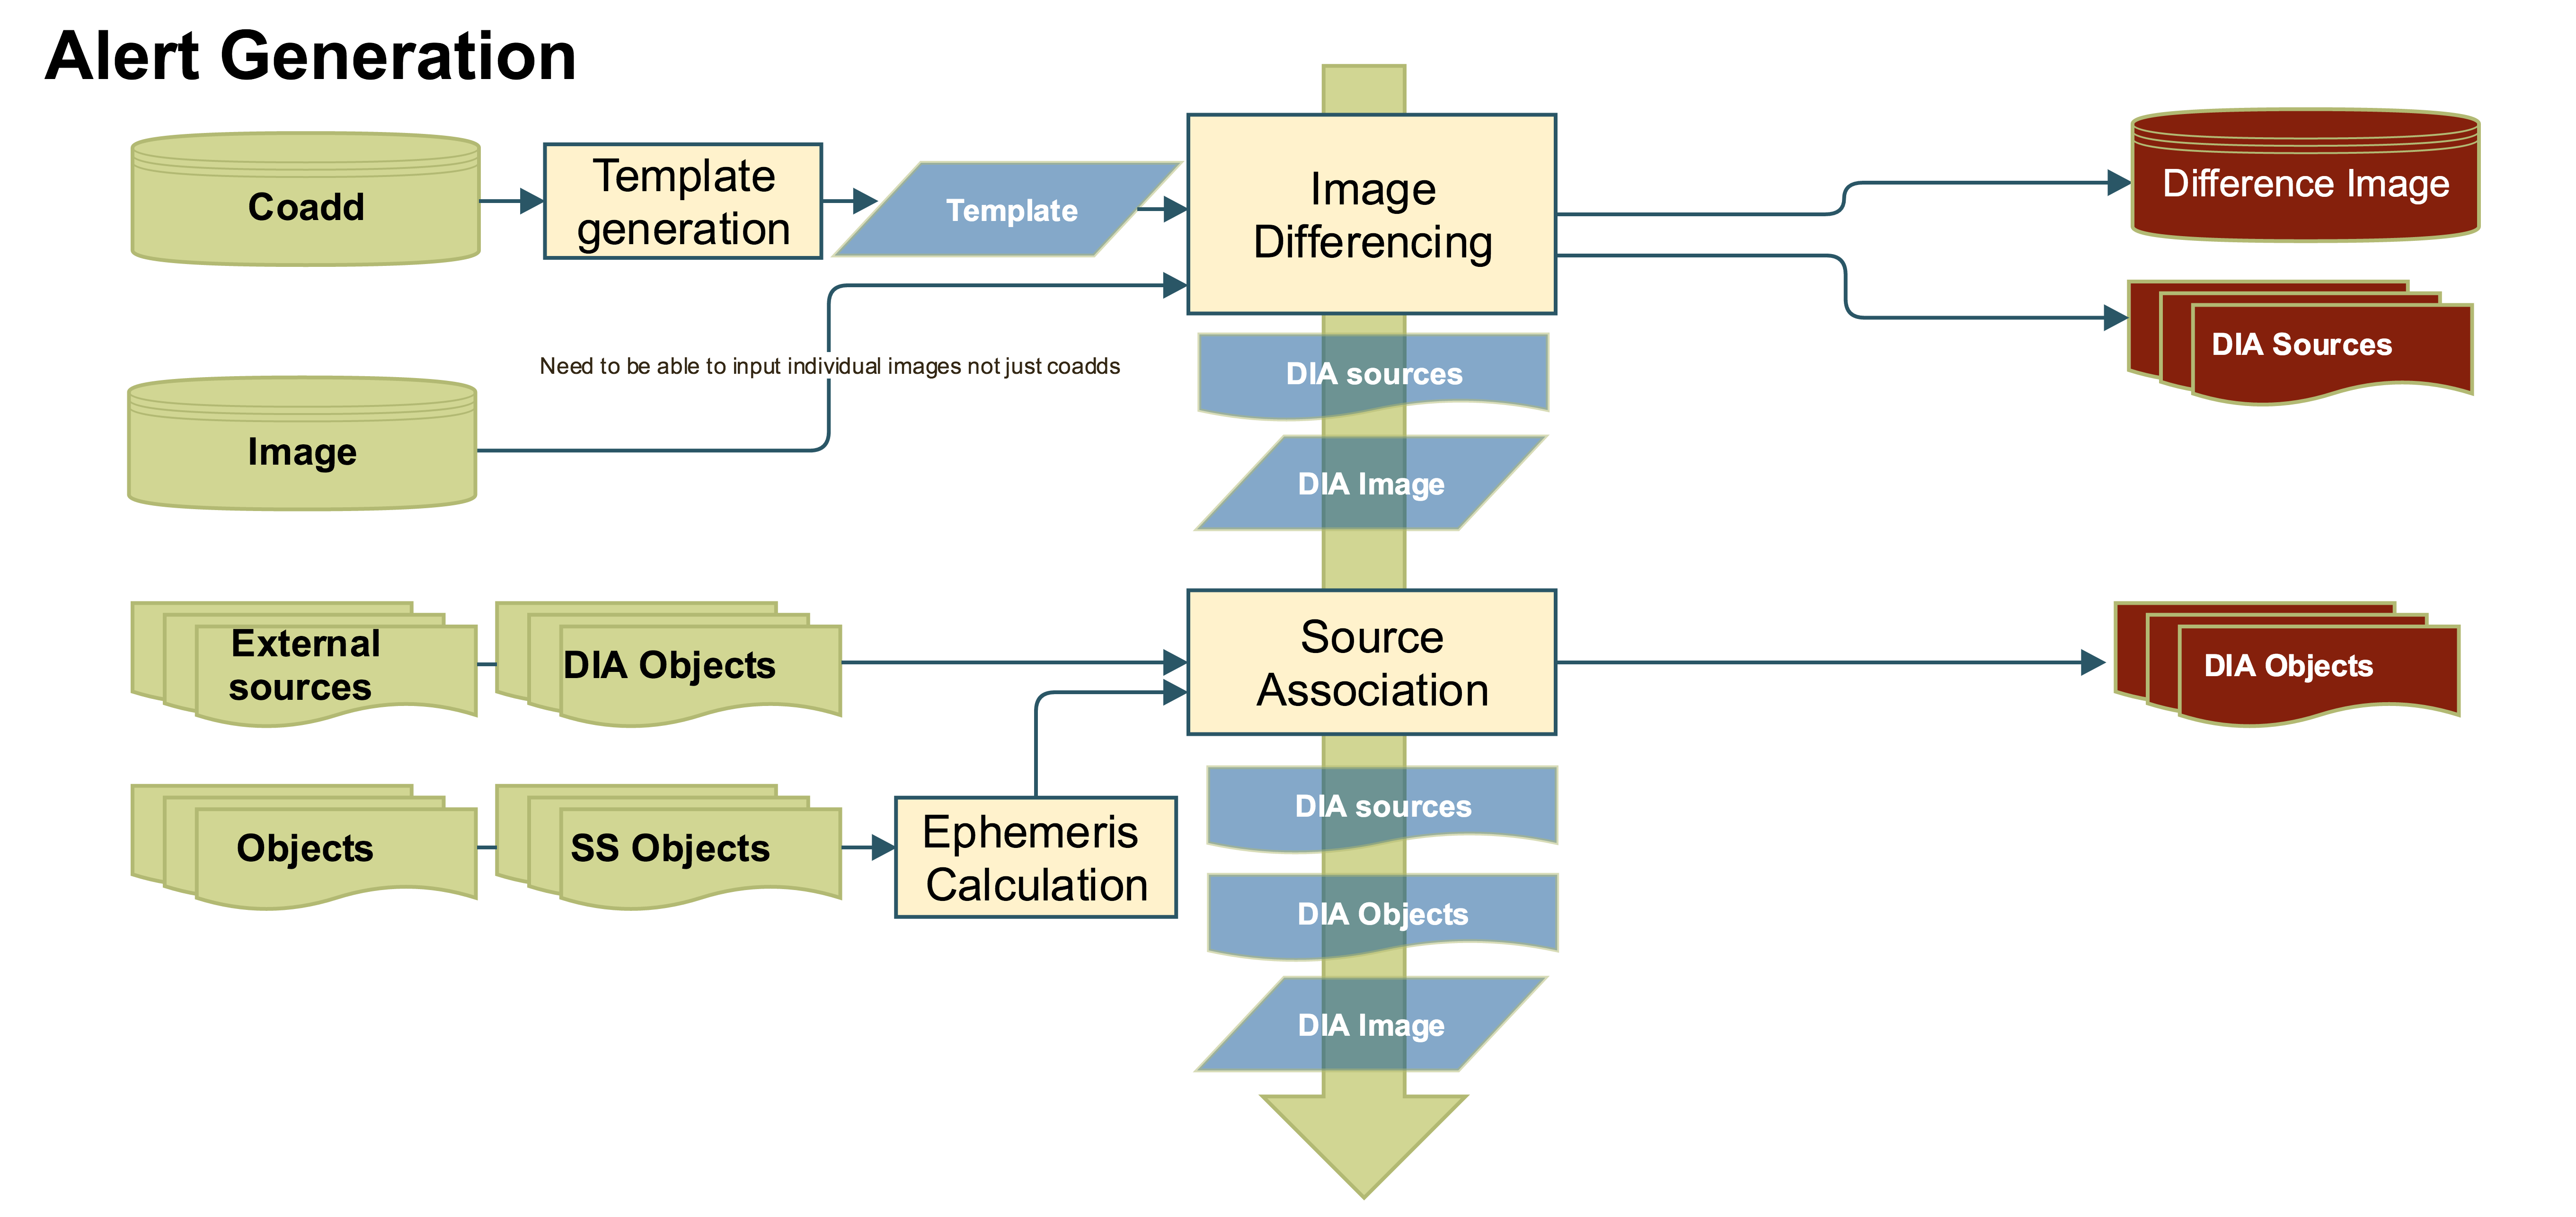
\includegraphics[width=0.9\textwidth]{figures/Alert_Generation.png}
\caption{\label{fig:apAlertgen} Generation of alerts from the nightly data: image differencing and measurement of the properties of the \DIASources, identification and filtering of spurious events, association of previously detected \DIAObjects and \SSObjects with the newly detected \DIASources. }
\end{center}
\end{figure}
\subsubsection{Input Data}
\label{sec:apAGInput}

\paragraph*{CalExp Images:} Calibrated exposure processed through \ref{sec:apSingleFrameProcessing} with associated WCS, PSF, mask, variance, and background estimation.

\paragraph*{Coadd Images:} TemplateCoadd images that spatially overlap with the CalExp images processed through \ref{sec:apSingleFrameProcessing}. This coadded image is optimized for image subtraction and is expected to be characterized in terms of a tract/patch/filter. Generation of this template may account for differential chromatic refraction or be generated for a limited range of airmass, seeing, and parallactic angles.

\paragraph*{Object Databases:} \Objects that spatially overlap with the CalExp images processed through \ref{sec:apSingleFrameProcessing}. This \Object catalog will provide the source list for determining nearest neighbors to the detected \DIASources.


\paragraph*{DIAObject Databases:} \DIAObjects that spatially overlap with the CalExp images processed through \ref{sec:apSingleFrameProcessing}. This \DIAObject catalog will provide the association  list against which the \DIASources will be matched.

\paragraph*{SSObject Databases:} The \SSObject list at the time of the observation. The \SSObject positions will be propagated to the date of the CalExp observations and will provide an association  list for cross-matching against the detected \DIASources to identify known Solar System objects.

\paragraph*{Reference classification catalogs:} Classification of \DIASources based on their morphological features (and possibly estimates of the local density or  environment associated with the \DIASource) will be undertaken prior to association in order to reduce the number of false positives. The data structures that define these classifications will be required as an input to this spuriousness analysis.



\subsubsection{Output Data}
\label{sec:apAGOutput}

\paragraph*{DiffExp Images:} Image differences derived by subtracting a TemplateCoadd from a CalExp image.

\paragraph*{DIASource Databases:} \DIASources detected and measured from the DiffExps using the set of parameters described in \DPDD will be persisted.


\paragraph*{DIAObject Databases:} \DIASource will be associated with existing \DIAObjects and persisted. New \DIASource (i.e.\ those not associated) will generate a new instance of a \DIAObject.


\subsubsection{Template Generation}
\label{sec:apCRTemplates}

Template generation requires the creation or retrieval (see \ref{sec:acRetrieveTemplate}) of a TemplateCoadd that is matched to the position and spatial extent of the input CalExp. Generation of the TemplateCoadd could be from a persisted Coadd that was generated from CalExp exposures with comparable (within a predefined tolerance) airmass and parallactic angles, or from a model that corrects for the effect of  differential chromatic refraction (see \ref{sec:acDCRTemplates}). It is expected that these operations would be undertaken on a CCD level but for efficiency the TemplateCoadd might be returned for a full focal plane or a series of \textit{patches}  or a \textit{tract}.


\paragraph{Pipeline Tasks}

\begin{itemize}
\item Query for a TemplateCoadd images that are within a given time interval of the CalExp  (default 2 years) of the current CCD image, and are within a specified airmass and parallactic angle.
\item (optional) Derive a seeing and DCR corrected TemplateCoadd from a model (see DCR template generation in \ref{sec:acDCRTemplates}). The current prototype approach assumes that the TemplateCoadd  will be derived for the zenith and will comprise a data cube with spatial and wavelength dimensions (a low resolution spectrum per pixel). Propagating to the observation will require aligning the DCR correction in the direction of the parallactic angle of the CalExp.
\end{itemize}

\subsubsection{Image differencing}

Image differencing incorporates the matching of a TemplateCoadd to a CalExp (astrometricly and in terms of image quality), subtraction of the template image, detection and measurement of \DIASources, removal of spurious \DIASources, and association of the \DIASources with previously identified \DIAObjects, and \SSObjects.

\paragraph{Pipeline Tasks}

\begin{itemize}
\item Determine a relative astrometric solution from the WCS of the TemplateCoadd image and CalExp image
\item Match the DRP \Sources for the TemplateCoadd (see \ref{sec:drpFinalImChar}) against \Sources from the SFM pipeline (see \ref{sec:apSingleFrameProcessing}) of the raw images.
\item Warp or resample the TemplateCoadd using a Lanczos filter  (as described in \ref{sec:spWarp}) to match the astrometry of the CalExp. It is possible that astrometricly matching the TemplateCoadd and CalExp using faint source will need to be undertaken dependent on the accuracy of the WCS.
\item For CalExp images with an image quality that is better than the TemplateCoadd preconvolve the CalExp image with the PSF. Use a  convolution kernel (see \ref{sec:spKernels}) that is matched to the source detection kernel. This reduces the need for deconvolution in the PSF matching (see \ref{sec:acImageSubtraction})
\item Match the PSF of the CalExp and TemplateCoadd images as described in \ref{sec:acDiffImDecorrelation} and construct a spatial model for the matching kernel. This approach may include matching to a common PSF through homogenization of the PSF (see \ref{sec:acPSFHomogenization}.
\item Apply the matching kernel to the TempCoadd and subtract the images to generate a DiffExp (as described in \ref{sec:acImageSubtraction}). Dependent on the relative signal-to-noise in the science and template image decorrelation of the template image due to the convolution of the template with a matching kernel may be necessary (see \ref{sec:acDiffImDecorrelation})
\item Detect \DIASources on the DiffExp using the algorithms described in \ref{sec:acSourceDetection}. Convolution with a detection kernel will depend on whether the CalExp was preconvolved in item 4.
\item Measurements of the \DIASources on the DiffExp will include dipole models and trailed PSF models (see  \ref{sec:acDipoleModels} and \ref{sec:acTrailedPointSourceModels} and parameters described in Table~2 of the \DPDD . The specific algorithms used for measurement of \DIASources will depend on whether the CalExp image was preconvolved.
\item Measurement of the PSF flux on snap difference images for all \DIASources.
\item The application of spuriousness algorithms, also known as ``real-bogus'', may be applied at this time dependent on whether the number of false positives is less than 50\% of the detected sources (see \ref{sec:acSpuriousnessAlgorithms})\footnote{The requirement for a 50\% false positive rate is given in the XXX and impacts the sizing model for the alert stream}. \DIASources classified as spurious at this stage may not be persisted (dependent on the density of the false positives). The default technique will be based on a trained random forest classifier. It is likely that the training of this classifier will need to be conditioned on the image quality and airmass of the observations.
\end{itemize}

\subsubsection{Source Association}
\label{sec:apSourceAssoc}

In Source Association \DIASources detected within a given CCD will be cross-matched or associated (see \ref{sec:acDIAObjectGeneration}) with the \DIAObject table and the \SSObjects (whose ephemerides have been generated for the time of the current observation). The association will be probabilistic  and account for the uncertainties within the positions. The association may include flux and priors on expected proper motions for the sources. External targets (e.g.\ well localized transient events from other telescopes or instruments) can be incorporated within this component of the nightly pipeline (essentially treating external sources as additional \DIAObjects and associating them with the \DIASources) enabling either matching to \DIASources or generation of forced photometry at the position of the external source.

\paragraph{Pipeline Tasks}

\begin{itemize}
\item Generate the positions of \SSObjects that overlap a DiffExp given its observation time by propagating the \SSObject orbit (see \ref{sec:acEphemerisCalculation})
\item As described in \ref{sec:acDIAObjectGeneration} source association will be undertaken for all \DIASources. Matching will be to \DIAObjects, and the ephemerides of \SSObjects. Positions for \DIAObjects will be based on a a time windowed (default 30 day) average of the \DIASources that make up the \DIAObject. A linear motion model for parallax and proper motion will be applied to propagate the \DIAObject to the time of the observation. A probabilistic association may need to account for one-to-many and many-to-one associations.  In dense regions it may be necessary to generate joint associations across all \DIAObjects (and associated \DIASources) in the local  vicinity of a \DIASource to correct for mis-assignment from previous observations. This could include the pruning and reassignment of \DIASources between \DIAObjects. A baseline approach for nightly processing will be to select based on a maximum a posteriori estimate for the association.
\item \DIASources will be positionally matched to the nearest 3 stars and 3 galaxies in the DRP \Object database. In its simplest case the search algorithm will be a tree-based nearest neighbor search (the default radius for association is not defined) . The matched \Objects will be persisted as a measure of local environment.
\item \DIASources unassociated with a \DIAObject will instantiate a new \DIAObject.
\item The aggregate positions for the \DIAObjects will be updated based on a rolling time window (default 30 days).
\item Proper motion and parallax of the \DIAObject will be updated using a linear model as described in \ref{sec:acStellarMotionFitting}.
%It is not currently clear if there is a science case for generating proper motions and parallaxes within the %DIAObjects if the DRP Objects are available for each source.
\end{itemize}


\clearpage

\subsection{Alert Distribution Pipeline (\wbsAP)}

The Alert Distribution Pipeline takes the newly discovered \DIAObjects (including their associated historical observations) and all related metadata as described in the \DPDD, and delivers alert packets in \VOEvent format to a variety of endpoints via standard IVOA protocols (eg., \VOEvent Transport Protocol; VTP\@). Packaging of the event will include the generation of postage stamp cutouts (30x30 pixels on average) for the difference image and the template image together with the variance and mask pixels for these cutouts.

The \SRD requires that the design of the LSST alert system should be able to handle 10$^7$ events per night, which corresponds to 10$^4$ alerts per visit or 50 alerts per CCD (with the time between subsequent visits averaging 39 seconds). All alerts (up to 10$^4$ per visit) must be transmitted within 60s of the closure of the shutter of the final snap within a visit.

For a nightly event rate of 10$^7$, and assuming the schema described in Tables 1 and 2 in the \DPDD together with the generation of the postage stamp cutouts, the compressed \VOEvents data stream amounts to approximately 600GB of data per night (assuming no filtering of the data).  The Alert Distribution pipeline is designed to distribute these alerts with a workflow, including the access point of external event brokers, shown in Figure~\ref{fig:apAlertDistribution}.

In addition to the full data stream the Alert Generation Pipeline will provide a basic alert filtering service. This service will run at the LSST U.S. Archive Center (at NCSA). It will enable astronomers to create filters (see  \ref{sec:apQueue}) that limit what alerts, and what fields from those alerts, are ultimately forwarded to them. These \emph{user defined filters} will be configurable with a simplified SQL-like declarative language. Access to this filtering service will require authentication by a user.

\VOEvent alerts will be persisted in an alert database as well as distributed through a message queue. The alert database (AlertDB) will be synchronized at least once every 24 hours and will be queriable by external users. The message queue that distributes the alerts is expected to have the capability  to replay events for the case of a break in the network connection between the queue and client but not to support general queries.

\begin{figure}[th]
\begin{center}
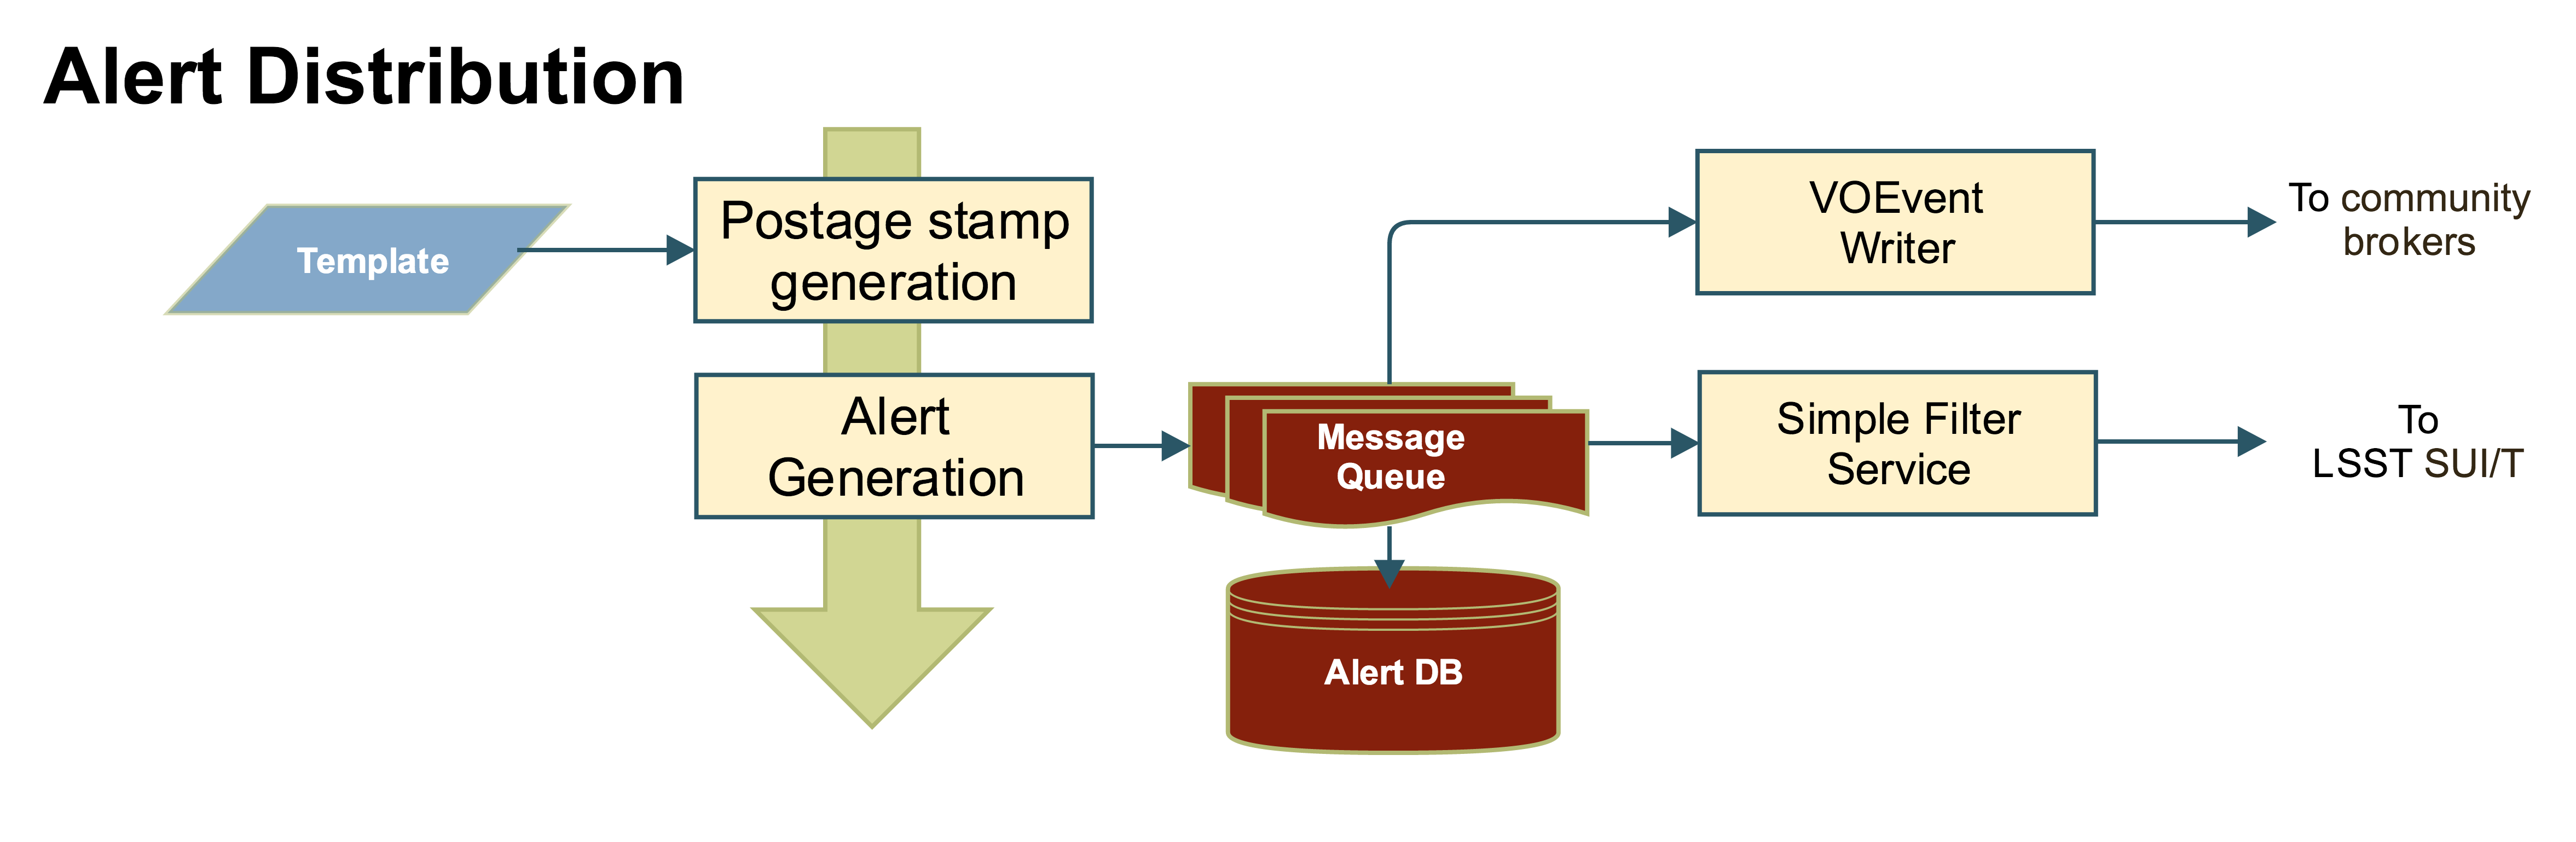
\includegraphics[width=0.9\textwidth]{figures/Alert_Distribution.png}
\caption{\label{fig:apAlertDistribution} Distribution of alerts from the nightly processing: generation of postage stamps around each detected \DIASource, distribution of the \DIAObjects as VOEvents, simple filtering of the event stream, and persistence of the events in a database.}
\end{center}
\end{figure}

\subsubsection{Input Data}
\label{sec:apADInput}

\paragraph*{DIAObject Database:} \DIAObjects, with new \DIASources, generated through image differencing will be used to create alert packets.

\paragraph*{Difference Images:} The DiffExp will be used to  generate postage stamp (cut-out) images of \DIASources within the CCD.

\paragraph*{Coadd Images:} The TemplateCoadd used in image subtraction will be used to  generate postage stamp images of the template image for \DIAObjects.


\subsubsection{Output Data}

\paragraph*{\VOEvent Database:} \VOEvents generated from the \DIAObjects and cutouts will be persisted within a database (e.g.\ a noSQL database) or object store.




\subsubsection{Alert postage stamp generation}

Creates the associated image cutouts (30x30 pixels on average) for all detect \DIAObjects (cutouts are generated from the current observation and not from historical observations).

\paragraph{Pipeline Tasks}

 \begin{itemize}
\item Extract from the DiffExp the cutout of each \DIAObject with a \DIASource detected within the current observation.  Cutout images will be scaled to the size of the \DIASource but on average will be 30x30 pixels. Variance and mask planes, WCS, background model, and associated metadata will be persisted. The prototype implementation assumes that these cutouts will be persisted as FITS images with a projection that is the  native projection of the DiffExps.

\item Extract from the TemplateCoadd  a cutout of each \DIAObject with a \DIASource detected within the current observation.  Cutout images will be identical in size and footprint as those derived from the DiffExp. Variance and mask planes, WCS, and associated metadata will be extracted with the pixel data. The prototype implementation assumes that these cutouts will be persisted as FITS imagesand that the projection will be that of  the DiffExps.
\end{itemize}

\subsubsection{Alert queuing and persistance}
\label{sec:apQueue}

The alert queue  distributes and persists \DIAObject with new \DIASources as \VOEvents through a message queue. It includes a \textit{limited} filtering interface but persists the full \VOEvents in an AlertDB. The event message stream and the AlertDB will be  synchronized at least once every 24 hours.


\paragraph{Pipeline Tasks}

\begin{itemize}
\item Publish \DIAObjects to a caching message queue (e.g.\ \href{http://kafka.apache.org}{Apache Kafka}) through the butler. The prototype implementation assumes a distributed and partitioned messaging system that uses a \href{https://en.wikipedia.org/wiki/Publish_subscribe_pattern}{publication-subscription} model for communication between clients and the queue. This model maintains feeds of messages in categories called topics. An example topic would be a \DIAObject. Whether a topic would comprise a full \DIAObject or a subset of the data remains open (passing subsets of parameters as individual topics would require that the client be able to synchronize and join topics into a full \DIAObject). For each of the 189 CCDs, approximately 50 events will be passed as messages to the messaging queuing system. The distribution of the events from a given CCD will not be synchronized with other CCDs within the focal plane (alerts from each CCD will be independently processed).

\item A consumer layer will subscribe to the  message queue and package them as \VOEvents and distribute these events to external users. To allow for network outages between the message queue and the consumer the message queue must be able to replay previous events.
\item  The consumer layer will provide a command line API to define simple queries or filters of the events (limited to querying on existing \DIAObject fields, or filtering the attributes of the \DIAObject). Web-based interfaces to the consumer layer will be developed by SUIT.
\item Filtered or the full stream of \DIAObjects will be packaged into \VOEvents and broadcast to VOEvent clients through the consumer layer
\item A full, unfiltered, VOEvent alert stream will be broadcast to the AlertDB using the consumer layer.
\item Prior to the start of the subsequent night's observations, the message queue will be flushed and synchronized with the AlertDB. It is possible to persist the message queue on longer timescale but it is a requirement hat synchronization be performed within 24 hours of the observations.
\end{itemize}

To cope with the variation in density of events as a function of position on the sky and the need for fault tolerance the message queue will need to be able to partition and replicate data. Given the 600GB of data generated per night from the alert distribution, each full \DIAObject stream will require about 0.1 Gb/s network capacity. Whether the consumer layer will instantiate a new consumer for each filter (or client) or will orchestrate the \VOEvents from a single subscription to the message queue is an open question that will depend on the expected network topology (internal and external to the data center at NCSA).

The AlertDB will have an interface that can be queried (to enable historical searches of events) including searches on other than timestamps. It is expected that the AlertDB will be a noSQL datastore (e.g.\ Cassandra).

%partitions must be ordered the same, failover must let a consumer to move to a different partion and have the messages ordered





\clearpage

\subsection{Precovery and Forced Photometry Pipeline}

The precovery and forced photometry  pipeline performs two tasks (see Figure~\ref{fig:apForcedPrecovery}). Forced PSF photometry is undertaken for all \DIAObjects that have a detected \DIASource within a, default 1 year, window of time from the observation.  Second, within 24 hours, precovery forced photometry is performed on all unassociated \DIASources within an image (i.e.\ new \DIAObjects). For each new \DIAObject, forced (PSF) photometry will be measured at the position of the source in each of the preceding  30-days of DiffExps.

Forced photometry is not required prior to alert generation. Completion of the precovery photometry is required within 24 hours of the completion of the observations. Forced and precovery can be undertaken as part of the nightly workflow if they do not impact the time required to distribute the alerts.

\begin{figure}[th]
\begin{center}
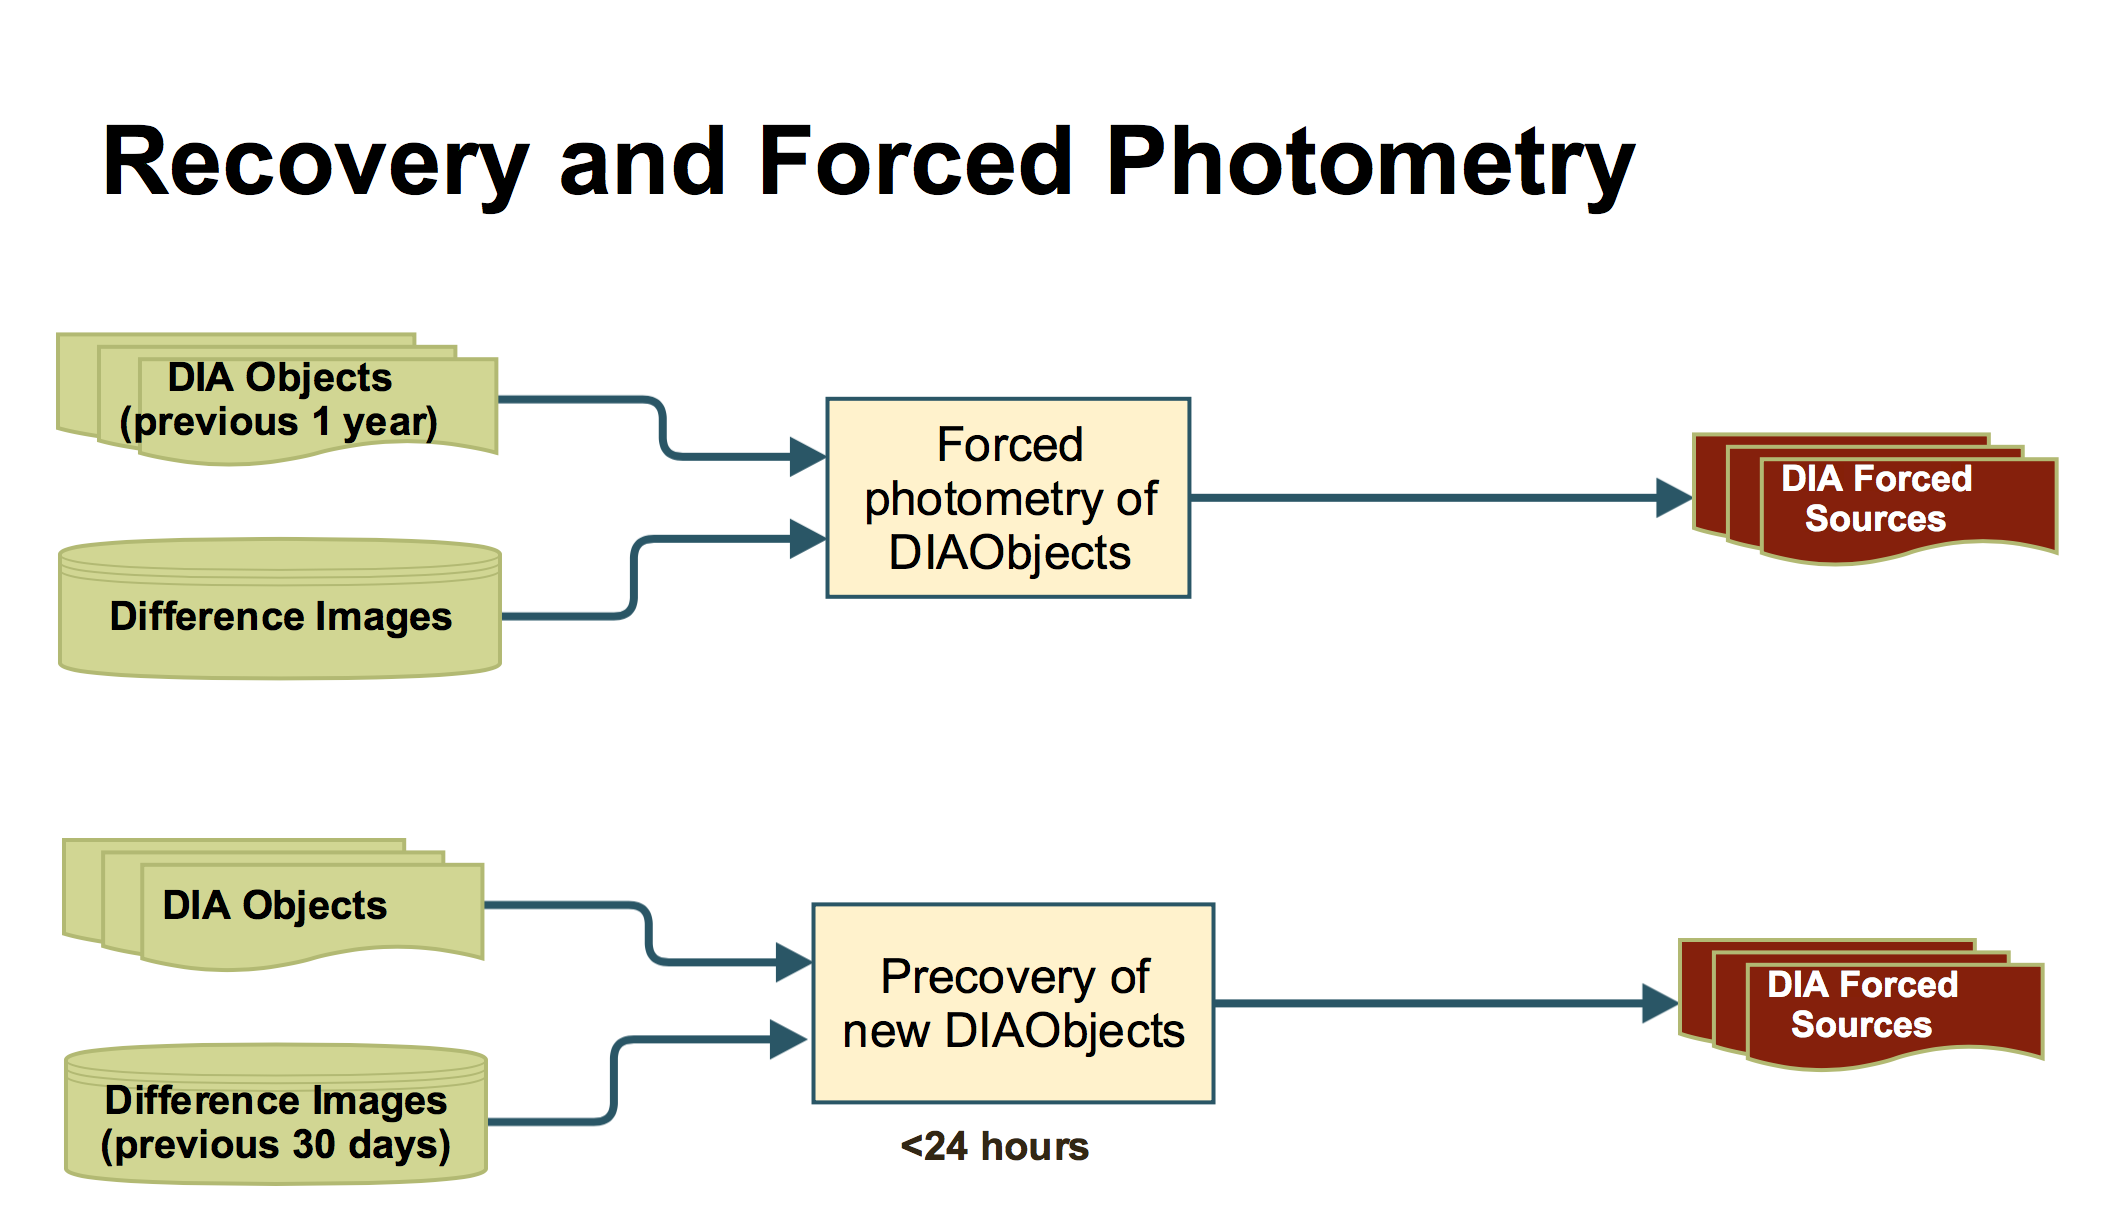
\includegraphics[width=0.9\textwidth]{figures/Forced_Precovery.png}
\caption{\label{fig:apForcedPrecovery} Forced photometry for \DIAObjects: forced photometry on a night's DiffExp for all \DIAObjects that have detected \DIASources within the last year, precovery photometry for the previous 30 days of DiffExps for new \DIAObjects}
\end{center}
\end{figure}

\begin{note}{For ZI: I moved the precovery to a single pipeline}\end{note}
\subsubsection{Input Data}

\paragraph*{Difference images:} A cache of DiffExps within a finite time interval (default 30 days) of the previous nights observations (inclusive of the previous nights data)

\paragraph*{DIAObject Database:} All \DIAObjects with a \DIASource detection within the last 12 months and all unassociated (new) \DIAObjects observed within the previous night

%\begin{note} We associate (measure forward) for 12 months but look back for 30 days\end{note}

\subsubsection{Output Data}

\paragraph*{DIAForcedSource Databases:} Forced PSF photometry at the centroid (from the aggregated individual \DIASource centroids) of a \DIAObject. The forced photometry is undertaken on the current night's DiffExp for all \DIAObjects with \DIASources detected within the last year, and on the previous 30 days of DiffExp for all newly detected \DIASources.


\subsubsection{Forced Photometry on all \DIAObjects}

Generate forced (PSF) photometry on the DiffExp for all \DIAObjects that overlap with the footprint of the CCD. Forced photometry is only generated for \DIAObjects for which there has been a \DIASource detection within the last 12 months. The forced photometry is persisted in the forced photometry table in the Level 1 database. Alerts are released prior to the generation of forced photometry and forced photometry is not released as apart of an alert which means that this component of the processing is not subject to the 60 second processing requirements for nightly processing.

\paragraph{Pipeline Tasks}

\begin{itemize}
\item Extract all \DIAObjects within the Level 1 database with a detected \DIASource within the last year (including the current nights observations). This information is available from the \DIASource and \DIAObject association.
\item For the aggregate positions within the \DIAObject undertake a PSF forced measurement as described in section \ref{sec:acForcedMeasurement}
\item Update the forced photometry tables in the Level 1 database.
\end{itemize}



\subsubsection{DIAObject Forced Photometry:}

Updated forced photometry table for all new \DIAObjects


\paragraph{Pipeline Tasks}

\begin{itemize}
\item Extract from the Level 1 database all \DIAObjects that were unassociated (i.e.\ new \DIASource detections) from the previous nights reduction. Filtering of the \DIAObjects will need to account for cases where new \DIASources are observed more than once within a night (where the second or subsequent observations do not result in a new \DIAObject).
\item Extract DiffExps within a  default 30 day window prior to the observation
\item Force photometer the extracted images as described in \ref{sec:acForcedMeasurement} using a PSF model and the centroid defined in the \DIAObject
\item Update the forced photometry table within the Level 1 database
\end{itemize}
\clearpage



\subsection{Moving Object Pipeline (\wbsMOPS)}
\label{sec:apMovingObjectPipeline}

The Moving Object Pipeline (MOPS) is responsible for generating and managing the Solar System data products. These are Solar System objects with associated Keplerian orbits, errors, and detected \DIASources. Quantitatively, it shall be capable of detecting 95\% of all Solar System objects that meet the criteria specified in the \OSS\@ (i.e.\ the observations required to define an orbit). Each visit within 10 degrees of the Ecliptic will detect approximately 4,000 asteroids.

Components of MOPS are run during and separately from nightly processing (see Figure~\ref{fig:apMOPS}). MOPS for nightly processing is described in \ref{sec:apSourceAssoc} as part of source association. ``Day MOPS'' processes newly detected \DIAObjects to search for candidate asteroid tracks. The procedure for Day-MOPS is to link \DIASource detections within a night (called tracklets), to link these tracklets across multiple nights (into tracks), to fit the tracks with an orbital model to identify those tracks that are consistent with an asteroid orbit, to match these new orbits with existing \SSObjects, and to update the \SSObject table. By its nature this process is iterative with \DIASources being associated and disassociated with \SSObjects. It is expected that a frequency of one day for these iterations (i.e.\ the \SSObjects will be update each day) will be sufficient.

\begin{figure}[th]
\begin{center}
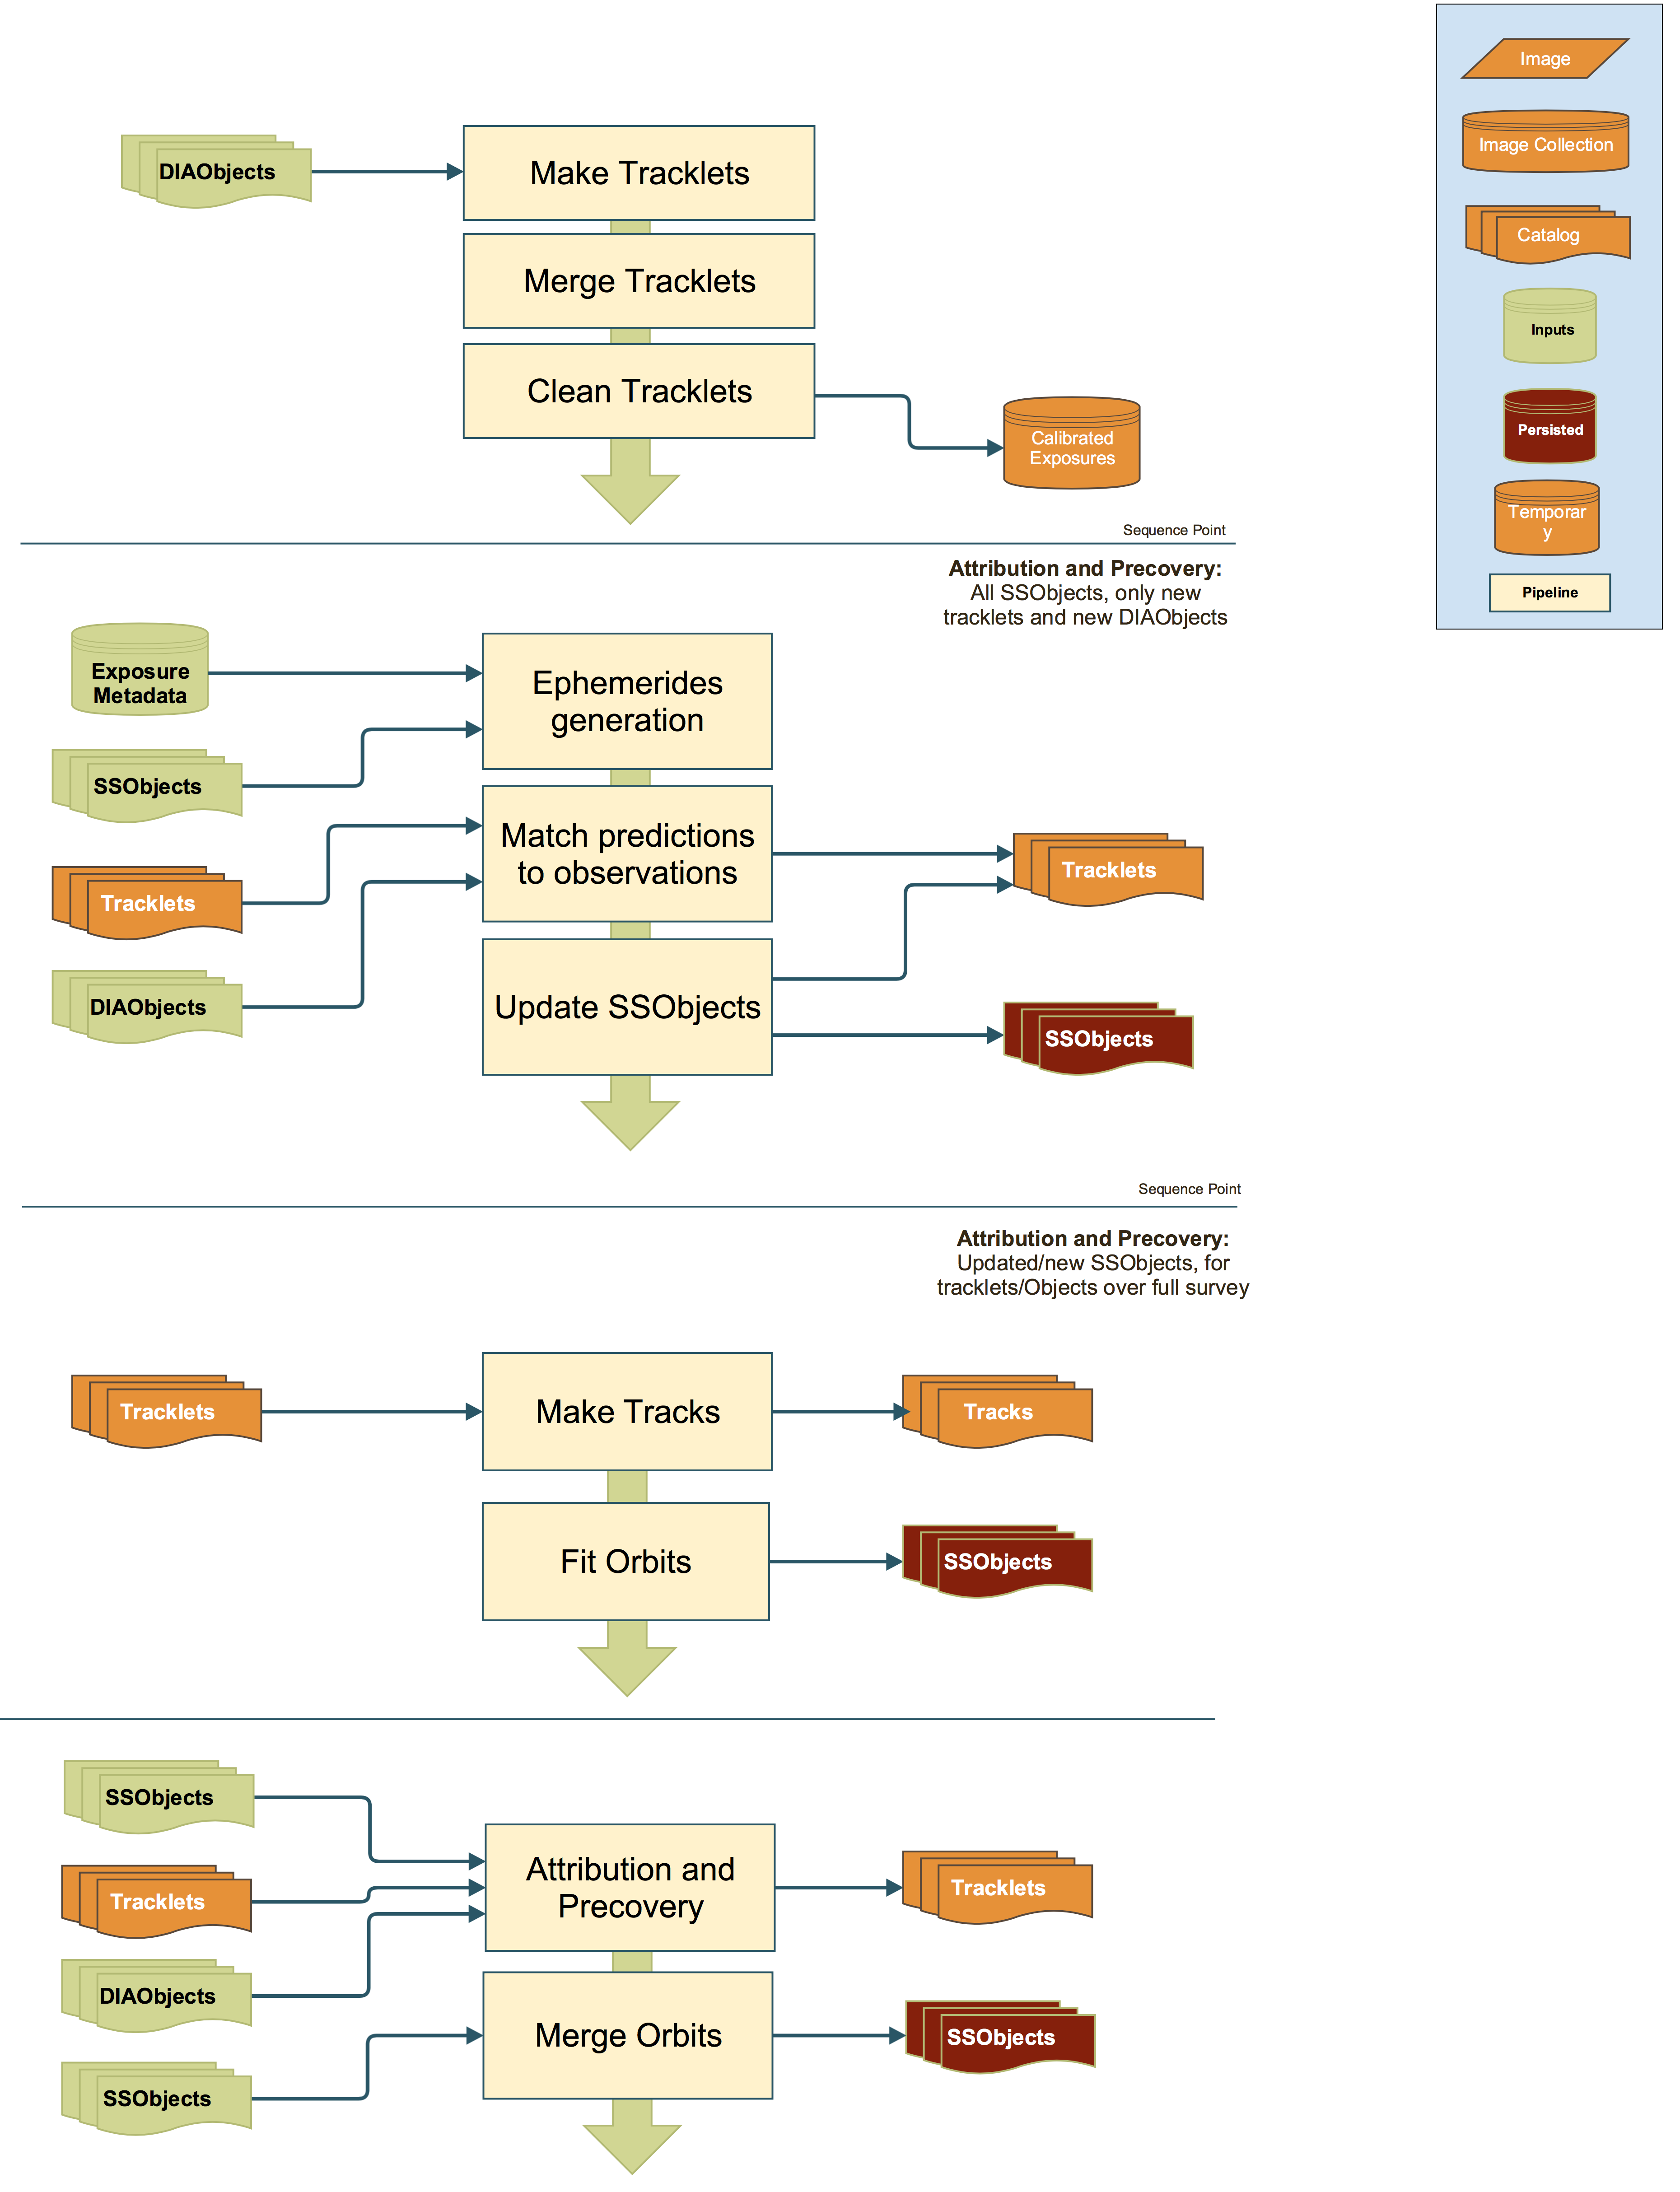
\includegraphics[width=0.9\textwidth]{figures/MOPS.png}
\caption{\label{fig:apMOPS} Detection and orbital modelling of moving sources within the nightly data: Tracklet generation from revisits, filtering of tracklets based on  known \SSObjects, fitting of tracks and orbits to tracklets, pruning of tracklets and \DIAObjects based on new and updated \SSObjects.}
\end{center}
\end{figure}

\subsubsection{Input Data}

\paragraph*{DIAObject Database: } Unassociated \DIASources from the previous night of observing.  This means \DIAObjects that were newly created during the previous night because they could not be associated with known \DIAObjects.  \DIASources associated with an \SSObject in the night are still passed through the MOPS machinery

\paragraph*{SSObject Database: } The catalog of known solar system sources

\paragraph*{Exposure Metadata:} A description of the footprint of the observations including the positions of bright stars or a model for the detection threshold as a function of position on the sky (including gaps between chips)


\subsubsection{Output Data}

\paragraph*{SSObject Database: } An updated \SSObject database with \SSObjects both added and pruned as the orbital fits are refined

\paragraph*{DIASource Database:} A updated \DIASource database with \DIASources assigned and unassigned to \SSObjects

\paragraph*{Tracklet Database:} A temporary database of tracklets measured during a night. This database will be persisted for at least a lunation.

\subsubsection{Tracklet identification}

From multiple visits within a night, link unassociated \DIASources to form tuples (or n-tuples) of \DIASources

\paragraph{Pipeline Tasks}

\begin{itemize}
\item Extract unassociated \DIASources from the Level 1 database
\item Link \DIASources into tracklets assuming a maximum velocity for the moving sources. The maximum velocity will be based on a prior as described in  \cite{2007ASPC..376..395K}. For each tracklet a velocity vector will be calculated to enable pruning or merging of degenerate tracklets within a data set.
\item Merge tracklets by clustering in velocity and position (propagated to a common visit time). Tracklets can contain multiple points and all permutations of the asteroid tuples will be stored. In the process of merging tracklets \DIASources that are not a good fit for the merged tracklet will be remove and their associated tracklets returned to the tracklet database.  Moving or trailed sources will incorporate the position angle of the source when linking. Details of the implementation of the \DIASource linkage is described in \ref{sec:acMakeTracklets}
\item Temporarily persist a database of tracklets. This database will be required for at least 30 days of data but, depending on resources available, may persist for longer.
\end{itemize}


\subsubsection{Precovery and merging of tracklets}

Tracklets are matched and merged with existing \SSObjects and removed from the Tracklet database. This culls any tracklets or \DIASources that obviously belong to an existing \SSObject from the rest of the processing.

\paragraph{Pipeline Tasks}

\begin{itemize}
\item Return all tracklets identified within a given night of observations
\item Return the footprints of each visit and the time of the observation
\item Extract \SSObjects from the \SSObject database and propagated those orbits to the position and time of a visit. Details of this orbit propagation for precovery are described in \ref{sec:acEphemerisCalculation}.
%\begin{note}What are the numbers for the \SSObject propagation and number of tracklets per visit\end{note}
\item Merge (precovery) the tracklets with the projected \SSObject trajectories and refit  the \SSObject orbit model. \DIASources previously associated with an \SSObject may no longer fit the updated \SSObject orbits. These \DIASources will be removed from the \SSObject and returned as unassociated \DIAObjects to the level 1 database. All tracklets associated with these \DIAObjects will be  returned to the tracklet database. Details of this attribution and precovery are described in \ref{sec:acAttributionAndPrecovery}
\end{itemize}

\subsubsection{Linking tracklets and orbit fitting}

Given a database of tracklets constructed from a window (default 30 days) of time, link the tracklets into tracks assuming a quadratic approximation to the trajectory. Fit these tracks with orbital models and update the \SSObject database.

\paragraph{Pipeline Tasks}

\begin{itemize}
\item Extract all tracklets from the tracklet database for a specified window in time (default 30 days)
\item Merge tracklets into tracks based on their velocities and accelerations. Candidate tracks are pruned by fitting a quadratic relation to the positions (after applying a topocentric correction to the positions of the sources). Efficiency in this matching procedure is provided by a spatial index such as a kd-tree (see \ref{sec:acOrbitFitting}).
\item Fit an orbit to each candidate track using a tool such as OOrb \\(https://github.com/oorb/oorb) and, for poorly fitting  points, return the \DIASources and associated tracklets to their respective databases for subsequent reprocessing.
\item Merge \SSObjects that have similar orbital parameters based on range searches within the six dimensional orbital parameter space.  Merged \SSObjects will need to be refit and any poorly fitting \DIASources (and associated tracklets) returned  to their respective databases for subsequent reprocessing. Details of this procedure are given in \ref{sec:acOrbitMerging}
\end{itemize}

\subsubsection{Global precovery}

For all new or updated \SSObjects propagate the orbits to the positions and times of the observations of all tracklets and orphan \DIAObjects to ``precover'' further support for the orbits. This will prune the number of tracklets and \DIAObjects that will require merging in subsequent observations.

\paragraph{Pipeline Tasks}

\begin{itemize}
\item Return all tracklets identified within a given night of observations
\item Return the footprints of each visit and the time of the observation
\item Extract orbits for all new or updated \SSObjects and propagate the positions to the times of the observations for all visits covering the extent of the tracklet database, default 30 days, (see \ref{sec:acEphemerisCalculation})
\item Merge the tracklets with the projected \SSObject positions and refit the \SSObject orbit model. Poorly fitting \DIASources (and associated tracklets) will be removed from the \SSObject and returned as unassociated \DIAObjects to the Level 1 database (as described in \ref{sec:acAttributionAndPrecovery}).
\end{itemize}


The process for precovery and updating of the \SSObject models is naturally iterative (given the pruning of poorly fitting \DIAObjects and tracklets). Updates of the \SSObjects as part of each night of operations should enable sufficient iterations without requiring Day-MOPS to be rerun multiple times per day. The computationally expensive operations in this pipeline are the orbit propagation and the orbit fitting. Resources required for orbit propagation could be reduced be removing the initial precovery stage but at the cost of increasing the number of tracklets that would be available for matching into tracks. Orbital trajectories could be pre-calculated and modelled as polynomials to enable fast interpolation during Day-MOPS.



Extending the Global Precovery to include singleton \DIASources (i.e.\ one that are not merged into tracklets) would enable the identification of asteroids at the edge of the nightly footprint (where an object moves outside of the nightly survey footprint prior to the second visit or a second visit is not obtained for a given field).

\subsubsection{Prototype Implementation}

Prototype MOPS codes are available at \url{https://github.com/lsst/mops_daymops} and \url{https://github.com/lsst/mops_nightmops}. Current DayMOPS prototype already performs within the computational envelope envisioned for LSST Operations, though it does not yet reach the required completeness requirement.
